\begin{mainquestion}{nonidealinductor}{Non-Ideal Inductor Bode Plot}

\questionpoints

A practical inductor can be modeled using a series resistance $R_s$ (RDC), 
an inductance $L$, and a parasitic capacitance $C_p$ in parallel with the series branch.

\begin{center}
\begin{circuitikz}
    \draw (0,0) to[short, o-] (1,0)
          to[L=$L$] (3,0)
          to[R=$R_s$] (5,0)
          to[short, -o] (6,0);
    \draw (1,0) to[short] (1,-2)
          to[C=$C_p$] (5,-2)
          to[short] (5,0);
\end{circuitikz}
\end{center}

%--------------------------------------

% =========================================================
\begin{partquestion}{impedance}
{Derive the expression for the impedance $Z(j\omega)$ of the non-ideal inductor model.}

\begin{answer}
The impedance of the series branch is
\[
Z_s = R_s + j\omega L,
\]
and the impedance of the parasitic capacitor is
\[
Z_C = \frac{1}{j\omega C_p}.
\]
Since these two impedances are in parallel,
\[
Z(j\omega)=\frac{Z_s Z_C}{Z_s+Z_C}.
\]
Substituting and multiplying numerator and denominator by $j\omega C_p$ gives a simpler form:
\begin{align*}
Z(j\omega)
&=
\frac{(R_s+j\omega L)\frac{1}{j\omega C_p}}
{R_s+j\omega L+\frac{1}{j\omega C_p}}\\[6pt]
&=
\frac{R_s+j\omega L}
{1+j\omega C_p(R_s+j\omega L)}\\[6pt]
&=
\frac{R_s+j\omega L}
{(1-\omega^2 L C_p)+j\omega R_s C_p}.
\end{align*}
\end{answer}

%--------------------------------------
\end{partquestion}

% =========================================================
\begin{partquestion}{selfresonance}
{Derive the self-resonant frequency (SRF) of the inductor.}

\begin{answer}
At self-resonance, the reactive (imaginary) part of the impedance is zero. Using the expression for $Z(j\omega)$ derived in part (a):
\[
Z(j\omega) = \frac{R_s+j\omega L}{(1-\omega^2 L C_p)+j\omega R_s C_p}
\]
For the imaginary part of this total impedance to be zero, the phase of the numerator must equal the phase of the denominator. Equivalently, their imaginary-to-real ratios must be equal:
\[
\frac{\omega L}{R_s} = \frac{\omega R_s C_p}{1-\omega^2 L C_p}
\]
Assuming $\omega \neq 0$, we can cancel $\omega$ and cross-multiply to solve for the exact resonance condition:
\begin{align*}
L(1-\omega^2 L C_p) &= R_s^2 C_p \\[6pt]
L - \omega^2 L^2 C_p &= R_s^2 C_p \\[6pt]
\omega^2 L^2 C_p &= L - R_s^2 C_p
\end{align*}
Dividing by $L^2 C_p$ gives the exact self-resonant frequency:
\[
\omega_{0,\text{exact}} = \sqrt{\frac{1}{LC_p} - \left(\frac{R_s}{L}\right)^2}
\]
For a typical inductor where $R_s$ is small (specifically, when $(R_s/L)^2 \ll 1/(LC_p)$), the second term under the radical becomes negligible, leading to the standard approximation:
\[
1-\omega^2 L C_p = 0 \quad\Rightarrow\quad \omega_0 \approx \frac{1}{\sqrt{L C_p}}
\]
Thus, the exact and approximate frequencies are:
\[
\boxed{\omega_{0,\text{exact}} = \sqrt{\frac{1}{LC_p} - \left(\frac{R_s}{L}\right)^2}}
\qquad\text{and}\qquad
\boxed{\omega_0 \approx \frac{1}{\sqrt{L C_p}}}
\]

Either answer is acceptable.
\end{answer}

%--------------------------------------
\end{partquestion}

% =========================================================
\begin{partquestion}{bodemagnitude}
{Sketch the magnitude Bode plot of $|Z(j\omega)|$ and describe its behavior in the three frequency regions:
(i) $\omega \ll \omega_0$,
(ii) $\omega \approx \omega_0$,
(iii) $\omega \gg \omega_0$.}

\begin{answer}
(i) For $\omega \ll \omega_0$, the capacitor is effectively open ($|Z_C|\gg |Z_s|$), so
\[
Z(j\omega)\approx Z_s \approx R_s + j\omega L \approx j\omega L \quad (\text{if } \omega L \gg R_s).
\]
Magnitude rises with slope $+20$ dB/decade (inductive behavior).

\vspace{0.25cm}

(ii) Near $\omega \approx \omega_0$, the inductor and parasitic capacitor resonate, producing a peak in $|Z|$.
With $R_s\neq 0$, the peak is finite (damped) rather than infinite.

\vspace{0.25cm}

(iii) For $\omega \gg \omega_0$, the capacitor dominates ($|Z_C|\ll |Z_s|$), so the parallel combination is approximately
\[
Z(j\omega)\approx Z_C = \frac{1}{j\omega C_p}.
\]
Magnitude falls with slope $-20$ dB/decade (capacitive behavior).

\begin{center}
    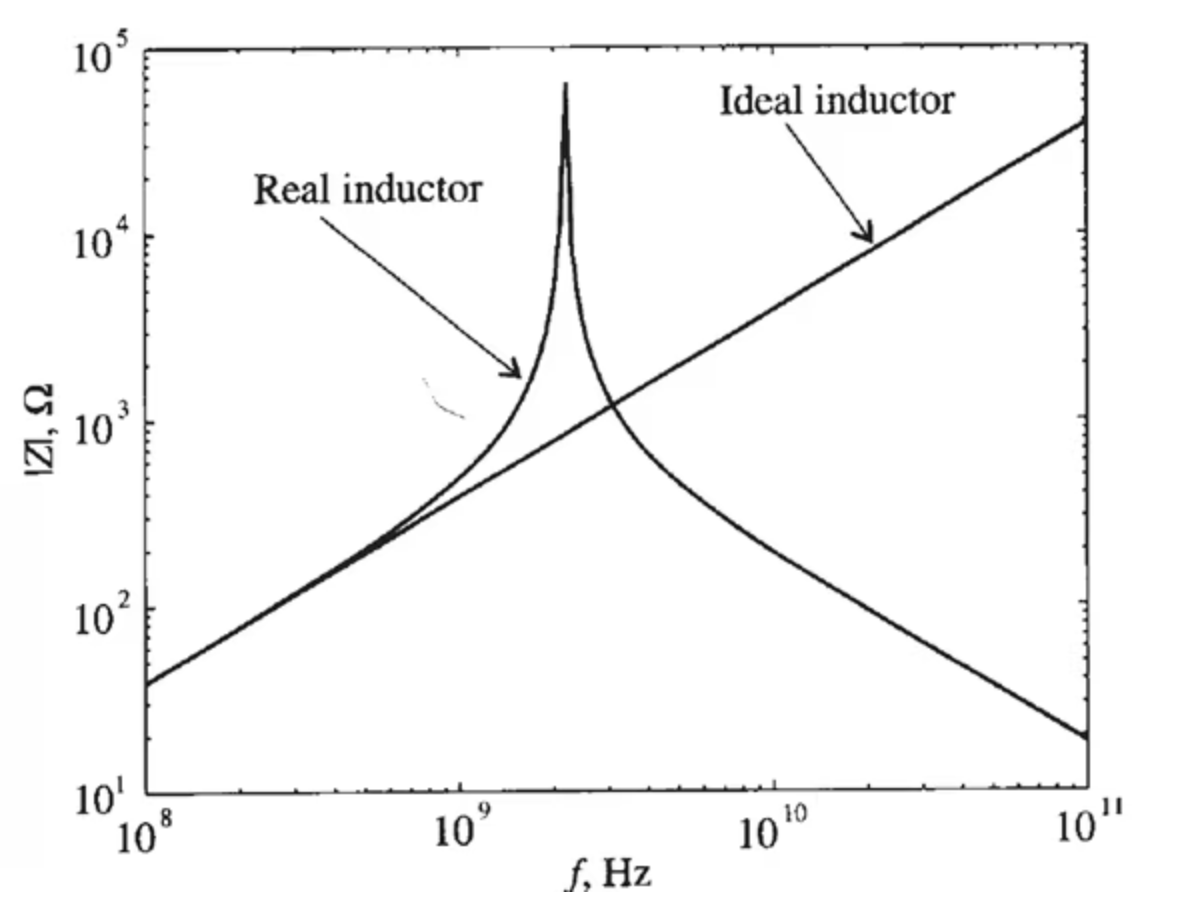
\includegraphics[width=0.6\textwidth]{q4.png}
\end{center}
\end{answer}

%--------------------------------------
\end{partquestion}

% =========================================================
\begin{partquestion}{qfactor}
{The Q-factor of the inductor at low frequency is defined as
\[
Q = \frac{\omega L}{R_s}.
\]
Explain how increasing $R_s$ affects the resonance peak in the magnitude Bode plot and the ability of the inductor to provide high impedance at RF (high) frequencies.}

\begin{answer}
Increasing $R_s$ lowers
\[
Q=\frac{\omega L}{R_s},
\]
so the resonance becomes more heavily damped: the peak magnitude at $\omega\approx\omega_0$ decreases and the peak becomes less sharp (broader).

At sufficiently high frequencies ($\omega\gg\omega_0$), the impedance is limited primarily by the parasitic capacitance:
\[
|Z(j\omega)| \approx \left|\frac{1}{j\omega C_p}\right|=\frac{1}{\omega C_p}.
\]
Thus, the loss of high impedance at RF is fundamentally due to $C_p$ providing a low-impedance shunt path. Increasing $R_s$ mainly affects the height/sharpness of the resonance peak; it does not remove the high-frequency roll-off set by $C_p$.
\end{answer}

\end{partquestion}

\end{mainquestion}
